\chapter{Phân tích yêu cầu và thiết kế hệ thống}

Chương này đi sâu vào việc phân tích các yêu cầu của ứng dụng MyBooksLibrary, từ đó xây dựng các biểu đồ Use Case và biểu đồ tuần tự nhằm mô hình hóa hành vi và luồng hoạt động của phần mềm.

\section{Phân tích yêu cầu}

\subsection{Yêu cầu chức năng}
Ứng dụng cần đáp ứng các chức năng cốt lõi sau để đảm bảo trải nghiệm đọc truyện trọn vẹn:
\begin{itemize}
    \item \textbf{Khám phá và tìm kiếm:} Hệ thống cho phép người dùng xem danh sách các truyện mới cập nhật, truyện phổ biến và tìm kiếm truyện theo từ khóa, thể loại hoặc tác giả.
    \item \textbf{Xem chi tiết và đọc truyện:} Hiển thị đầy đủ thông tin metadata của truyện (tóm tắt, đánh giá, trạng thái). Trình đọc (Reader) hỗ trợ tải trang truyện mượt mà, cho phép vuốt dọc hoặc ngang để chuyển trang.
    \item \textbf{Quản lý thư viện cá nhân:} Người dùng có thể lưu (bookmark) truyện yêu thích vào thư viện để dễ dàng theo dõi. Hệ thống tự động ghi nhận chương đang đọc dở để người dùng tiếp tục đọc ở lần mở ứng dụng sau.
    \item \textbf{Tải xuống ngoại tuyến:} Hỗ trợ tải các chương truyện về bộ nhớ cục bộ của thiết bị để có thể đọc khi không có kết nối mạng.
    \item \textbf{Đồng bộ dữ liệu:} Cho phép đăng nhập qua tài khoản Google để sao lưu và đồng bộ hóa thư viện cá nhân, lịch sử đọc lên máy chủ đám mây.
\end{itemize}

\subsection{Yêu cầu phi chức năng}
Bên cạnh các tính năng nghiệp vụ, hệ thống cần đảm bảo các tiêu chuẩn kỹ thuật sau:
\begin{itemize}
    \item \textbf{Hiệu năng:} Thời gian tải màn hình danh sách và nội dung trang truyện không được vượt quá 3 giây trong điều kiện mạng ổn định. Giao diện vuốt trang phải đạt 60 FPS (khung hình/giây).
    \item \textbf{Khả năng tương thích:} Ứng dụng phải hoạt động ổn định trên các thiết bị Android từ API level 30 (Android 11) trở lên, tự động điều chỉnh giao diện phù hợp với nhiều kích thước màn hình (điện thoại, máy tính bảng).
    \item \textbf{Tính khả dụng ngoại tuyến:} Các truyện đã tải xuống phải được truy xuất và đọc mượt mà ngay cả khi thiết bị ngắt kết nối Internet hoàn toàn.
    \item \textbf{Kiến trúc mã nguồn:} Mã nguồn phải tuân thủ nghiêm ngặt nguyên lý Clean Architecture và SOLID, giúp dễ dàng bảo trì và mở rộng tính năng sau này.
\end{itemize}

\section{Thiết kế hệ thống chi tiết}

\subsection{Sơ đồ Use Case tổng quát}
Sơ đồ Use Case thể hiện sự tương tác giữa người dùng (Người đọc) và hệ thống ứng dụng, cũng như sự giao tiếp của ứng dụng với các hệ thống bên ngoài (MangaDex API, Firebase).

\begin{figure}[H]
    \centering
    % TODO: Chèn ảnh Sơ đồ Use case tổng ở đây
    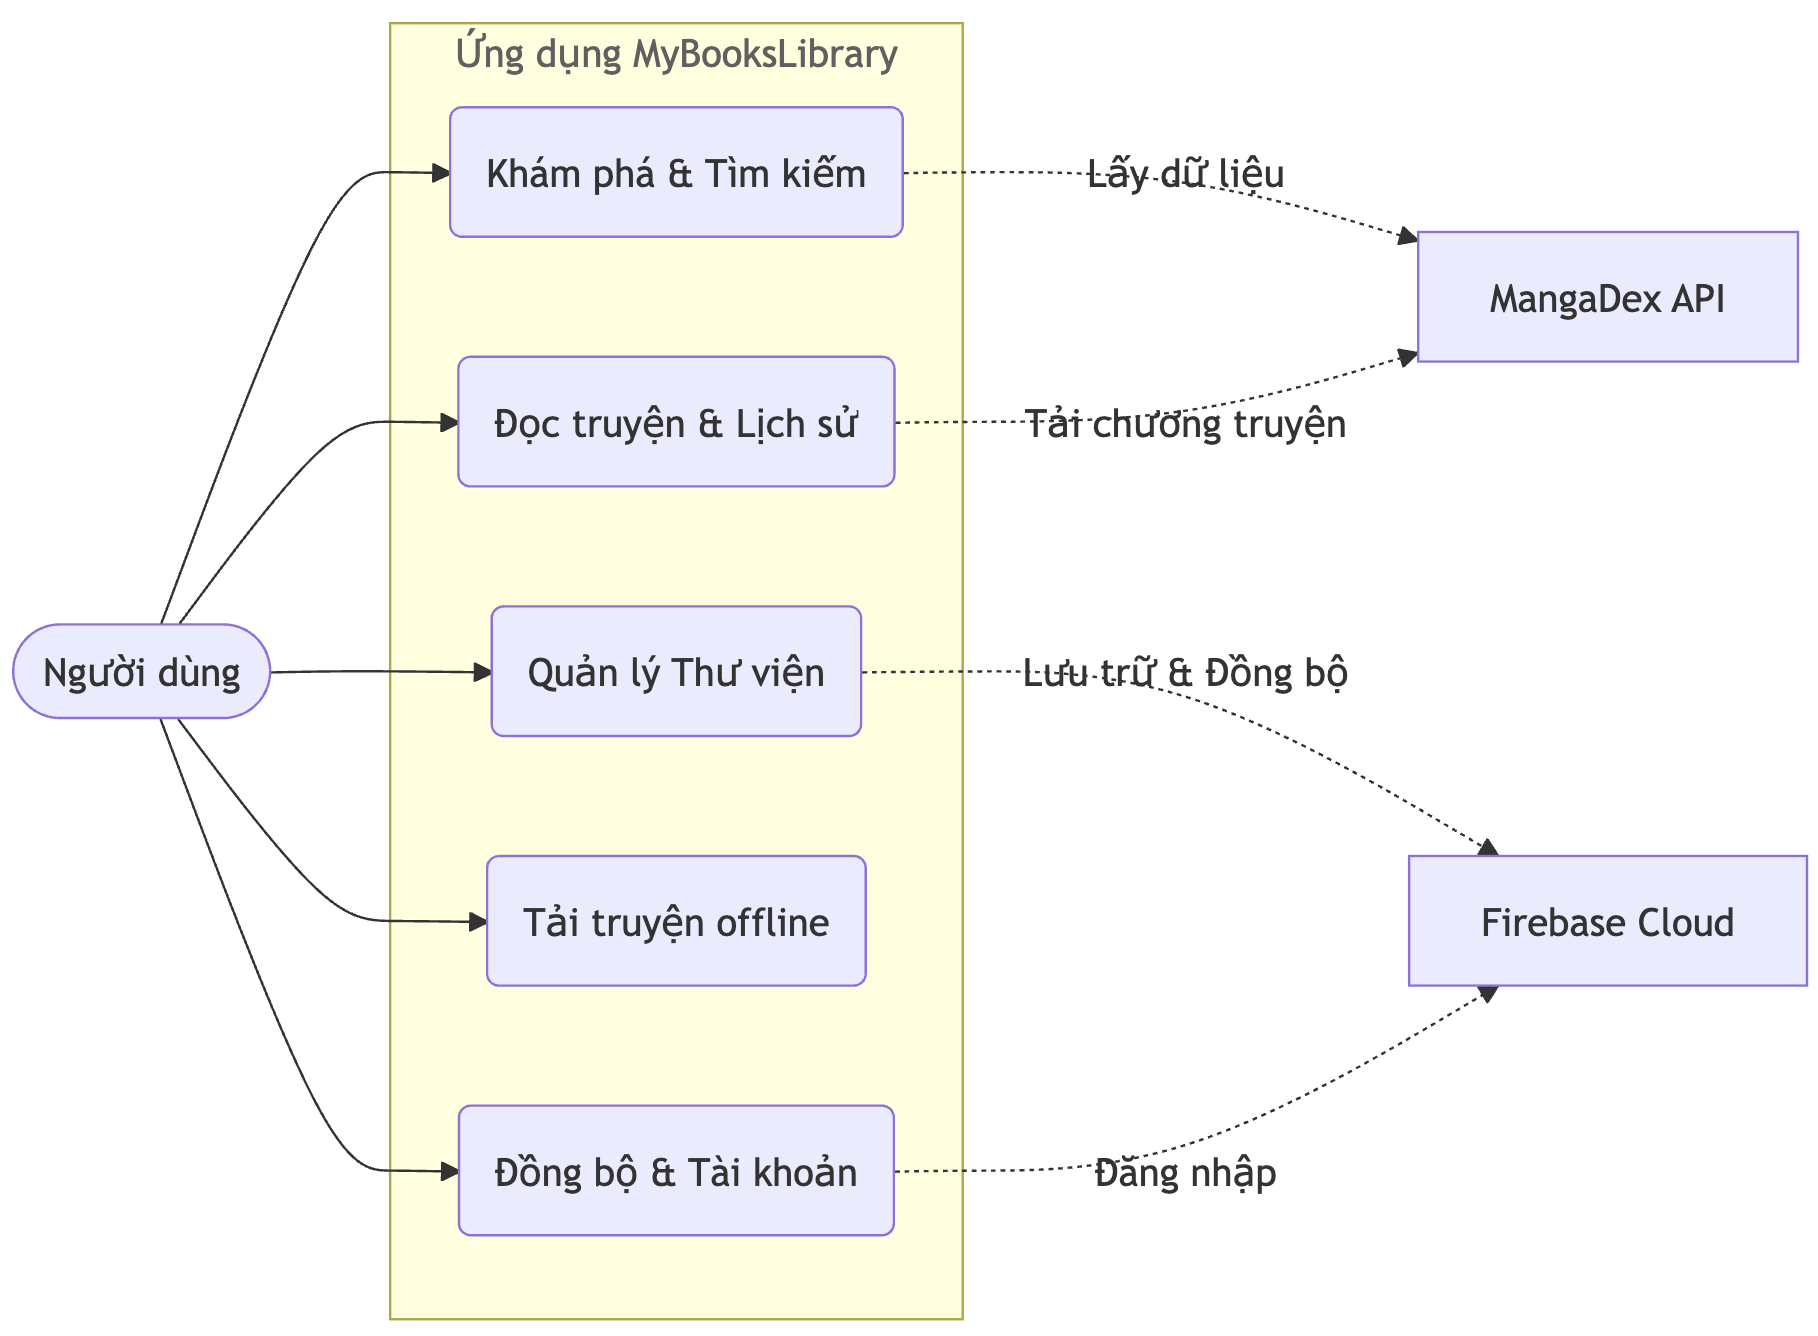
\includegraphics[width=0.8\textwidth]{figures/usecase_tong.png}
    \caption{Sơ đồ Use Case tổng quát của ứng dụng MyBooksLibrary}
    \label{fig:usecase_tong}
\end{figure}

\subsection{Đặc tả chi tiết các Use Case quan trọng}

Sau đây là đặc tả chi tiết cho 3 Use Case cốt lõi nhất của hệ thống, được trình bày thông qua bảng đặc tả.

% Bảng đặc tả Use Case 1
% \begin{table}[H]
%     \centering
%     \caption{Đặc tả Use Case: Khám phá và Tìm kiếm truyện}
%     \label{tab:uc_discover}
%     \begin{tabular}{|p{3.5cm}|p{11.5cm}|}
%     \hline
%     \textbf{Thuộc tính} & \textbf{Mô tả} \\ \hline
%     \textbf{Mã UC} & UC-01 \\ \hline
%     \textbf{Tên Use Case} & Khám phá và Tìm kiếm truyện \\ \hline
%     \textbf{Tác nhân} & Người dùng, MangaDex API \\ \hline
%     \textbf{Mô tả} & Cho phép người dùng duyệt qua danh sách các truyện thịnh hành, truyện mới cập nhật hoặc tìm kiếm truyện theo tên và bộ lọc. \\ \hline
%     \textbf{Tiền điều kiện} & Ứng dụng đã khởi động và có kết nối Internet ổn định. \\ \hline
%     \textbf{Hậu điều kiện} & Danh sách các bộ truyện (ảnh bìa, tên truyện) được hiển thị chính xác lên giao diện. \\ \hline
%     \textbf{Luồng cơ bản} & 
%     1. Người dùng mở ứng dụng, truy cập vào tab Khám phá hoặc Tìm kiếm. \newline
%     2. Người dùng nhập từ khóa hoặc chọn các bộ lọc (nếu có). \newline
%     3. Hệ thống gửi yêu cầu HTTP GET đến MangaDex API với các tham số tương ứng. \newline
%     4. API trả về chuỗi JSON chứa danh sách truyện. \newline
%     5. Hệ thống phân tích chuỗi JSON, lưu vào bộ đệm và hiển thị lên giao diện Compose. \\ \hline
%     \end{tabular}
% \end{table}

\begin{longtable}{|p{3.5cm}|p{11.5cm}|}
    \caption{Đặc tả Use Case: Khám phá và Tìm kiếm truyện} \label{tab:uc_discover} \\
    \hline
    \textbf{Thuộc tính} & \textbf{Mô tả} \\ \hline
    \endfirsthead % Đánh dấu kết thúc tiêu đề ở trang đầu tiên

    \hline
    \textbf{Thuộc tính} & \textbf{Mô tả} (tiếp theo) \\ \hline
    \endhead % Định nghĩa tiêu đề sẽ lặp lại khi sang trang mới

    \textbf{Mã UC} & UC-01 \\ \hline
    \textbf{Tên Use Case} & Khám phá và Tìm kiếm truyện \\ \hline
    \textbf{Tác nhân} & Người dùng, MangaDex API \\ \hline
    \textbf{Mô tả} & Cho phép người dùng duyệt qua danh sách các truyện thịnh hành, truyện mới cập nhật hoặc tìm kiếm truyện theo tên và bộ lọc. \\ \hline
    \textbf{Tiền điều kiện} & Ứng dụng đã khởi động và có kết nối Internet ổn định. \\ \hline
    \textbf{Hậu điều kiện} & Danh sách các bộ truyện (ảnh bìa, tên truyện) được hiển thị chính xác lên giao diện. \\ \hline
    \textbf{Luồng cơ bản} & 
    1. Người dùng mở ứng dụng, truy cập vào tab Khám phá hoặc Tìm kiếm. \newline
    2. Người dùng nhập từ khóa hoặc chọn các bộ lọc (nếu có). \newline
    3. Hệ thống gửi yêu cầu HTTP GET đến MangaDex API với các tham số tương ứng. \newline
    4. API trả về chuỗi JSON chứa danh sách truyện. \newline
    5. Hệ thống phân tích chuỗi JSON, lưu vào bộ đệm và hiển thị lên giao diện Compose. \\ \hline
\end{longtable}

% Bảng đặc tả Use Case 2
\begin{table}[H]
    \centering
    \caption{Đặc tả Use Case: Xem chi tiết và Đọc truyện}
    \label{tab:uc_read}
    \begin{tabular}{|p{3.5cm}|p{11.5cm}|}
    \hline
    \textbf{Thuộc tính} & \textbf{Mô tả} \\ \hline
    \textbf{Mã UC} & UC-02 \\ \hline
    \textbf{Tên Use Case} & Xem chi tiết và Đọc truyện \\ \hline
    \textbf{Tác nhân} & Người dùng, MangaDex API \\ \hline
    \textbf{Mô tả} & Người dùng chọn một truyện để xem thông tin chi tiết và truy cập vào giao diện đọc truyện (Reader) để duyệt qua các trang ảnh. \\ \hline
    \textbf{Tiền điều kiện} & Người dùng đã chọn được một bộ truyện từ danh sách. \\ \hline
    \textbf{Hậu điều kiện} & Cập nhật trạng thái và tiến độ đọc (chương số mấy, trang số mấy) vào cơ sở dữ liệu cục bộ. \\ \hline
    \textbf{Luồng cơ bản} & 
    1. Người dùng nhấn vào một bộ truyện. \newline
    2. Hệ thống gọi API để lấy thông tin chi tiết và danh sách các chương, hiển thị màn hình Chi tiết truyện. \newline
    3. Người dùng chọn một chương để đọc. \newline
    4. Hệ thống tải đường dẫn ảnh của chương đó qua At-Home API và hiển thị màn hình Đọc truyện. \newline
    5. Người dùng vuốt màn hình để chuyển trang. Coil tự động tải và hiển thị hình ảnh. \newline
    6. Khi người dùng thoát, hệ thống tự động lưu lại vị trí trang hiện tại vào Room Database. \\ \hline
    \end{tabular}
\end{table}

% Bảng đặc tả Use Case 3
\begin{table}[H]
    \centering
    \caption{Đặc tả Use Case: Quản lý Thư viện cá nhân}
    \label{tab:uc_library}
    \begin{tabular}{|p{3.5cm}|p{11.5cm}|}
    \hline
    \textbf{Thuộc tính} & \textbf{Mô tả} \\ \hline
    \textbf{Mã UC} & UC-03 \\ \hline
    \textbf{Tên Use Case} & Quản lý Thư viện cá nhân (Lưu truyện) \\ \hline
    \textbf{Tác nhân} & Người dùng \\ \hline
    \textbf{Mô tả} & Cho phép người dùng thêm các truyện đang theo dõi vào thư viện cá nhân để dễ dàng truy cập và nhận thông báo cập nhật. \\ \hline
    \textbf{Tiền điều kiện} & Đang ở màn hình Chi tiết truyện. \\ \hline
    \textbf{Hậu điều kiện} & Truyện được lưu thành công vào cơ sở dữ liệu Room cục bộ với trạng thái "Yêu thích". \\ \hline
    \textbf{Luồng cơ bản} & 
    1. Ở màn hình Chi tiết truyện, người dùng nhấn nút "Thêm vào Thư viện". \newline
    2. ViewModel nhận sự kiện và gọi xuống tầng Repository. \newline
    3. Repository thực hiện câu lệnh Insert/Update dữ liệu (Entity) của truyện vào bảng trong Room Database. \newline
    4. Flow theo dõi cơ sở dữ liệu phát ra tín hiệu thay đổi dữ liệu. \newline
    5. Giao diện tự động cập nhật, biểu tượng chuyển sang trạng thái "Đã lưu". \\ \hline
    \end{tabular}
\end{table}

\subsection{Luồng hoạt động chính (Sequence Diagrams)}

Để hiểu rõ hơn về cách các thành phần bên trong hệ thống (theo kiến trúc Clean Architecture) tương tác với nhau, phần này trình bày chi tiết luồng hoạt động của hai quy trình cốt lõi bằng biểu đồ tuần tự.

\subsubsection{Luồng lấy danh sách truyện từ MangaDex API}

Luồng hoạt động này mô tả cách dữ liệu di chuyển từ lúc người dùng tương tác với giao diện cho đến khi dữ liệu từ máy chủ bên ngoài được đưa về và hiển thị. 

\begin{figure}[H]
    \centering
    % TODO: Chèn ảnh Sơ đồ tuần tự lấy danh sách truyện
    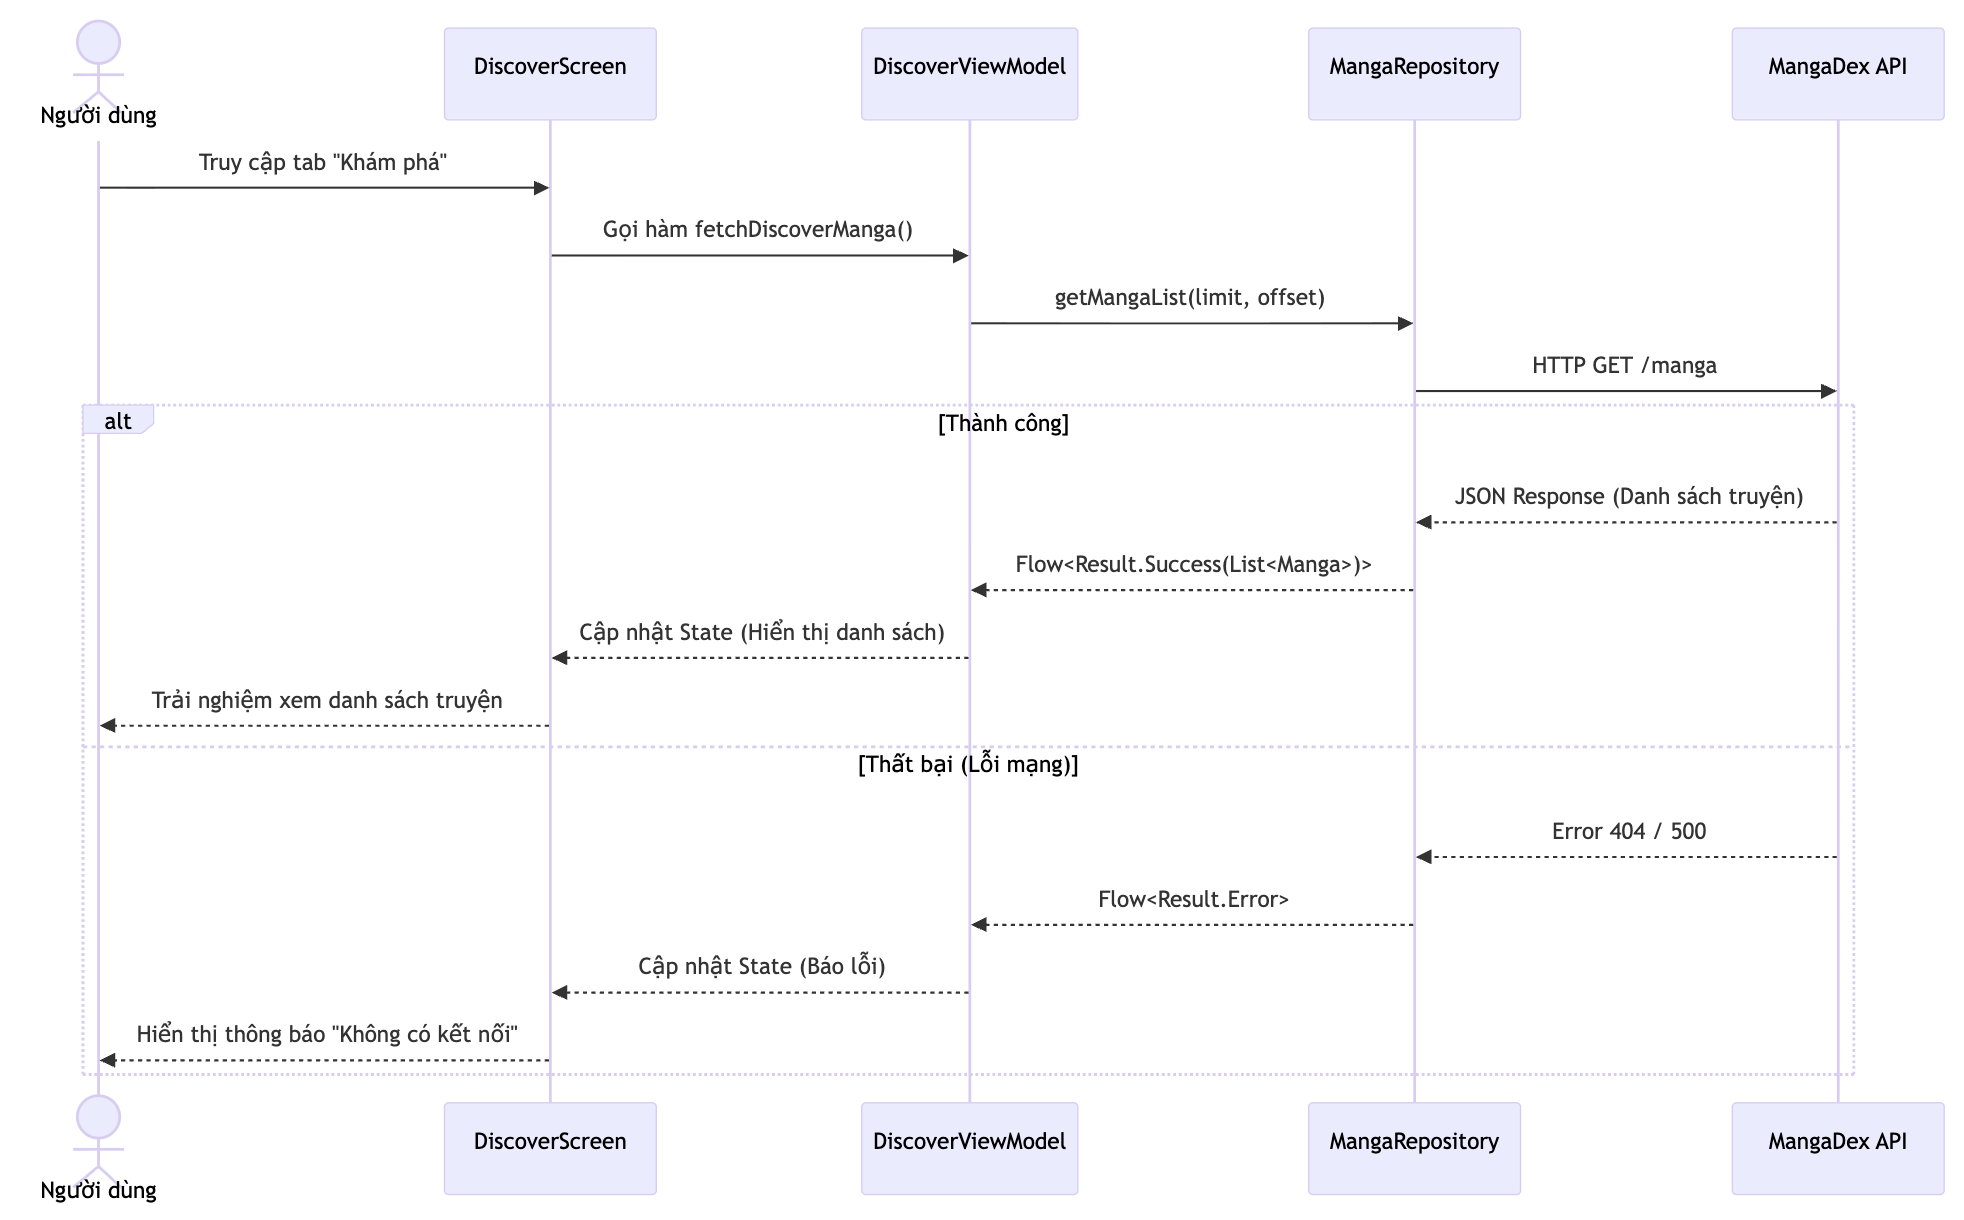
\includegraphics[width=0.9\textwidth]{figures/FetchListBookApi.png}
    \caption{Sơ đồ tuần tự: Luồng lấy danh sách truyện từ MangaDex API}
    \label{fig:seq_fetch_manga}
\end{figure}

\textbf{Giải thích chi tiết:}
Khi người dùng truy cập tab Khám phá, tầng \\ \texttt{UI (DiscoverScreen)} kích hoạt hàm \texttt{fetchDiscoverManga()} trong \texttt{DiscoverViewModel}. \texttt{ViewModel} này đóng vai trò xử lý logic Presentation, nó gọi xuống \texttt{MangaRepository} ở tầng Data để yêu cầu danh sách truyện. \texttt{Repository} sử dụng \texttt{MangaDexApi} (Retrofit) để thực hiện một HTTP GET request đến máy chủ. 
Nếu thành công, chuỗi JSON trả về được parse thành các Object \texttt{MangaListResponseDto}. \texttt{Repository} chuyển đổi Dto này thành \texttt{MangaModel} của tầng Domain và gửi kết quả về \texttt{ViewModel} thông qua \texttt{Flow<Result.Success>}. Cuối cùng, \texttt{ViewModel} cập nhật \texttt{UI State}, và Jetpack Compose phản ứng lại bằng cách recompose để hiển thị danh sách truyện lên màn hình. Trong trường hợp lỗi mạng, một \texttt{Result.Error} sẽ được trả về để hiển thị thông báo lỗi.

\subsubsection{Luồng lưu truyện vào thư viện local bằng Room}

Luồng này mô tả thao tác lưu trữ dữ liệu hoàn toàn ở bộ nhớ cục bộ, bảo đảm tính tức thời và cho phép ứng dụng phản hồi ngay lập tức cho người dùng.

\begin{figure}[H]
    \centering
    % TODO: Chèn ảnh Sơ đồ tuần tự lưu truyện vào thư viện
    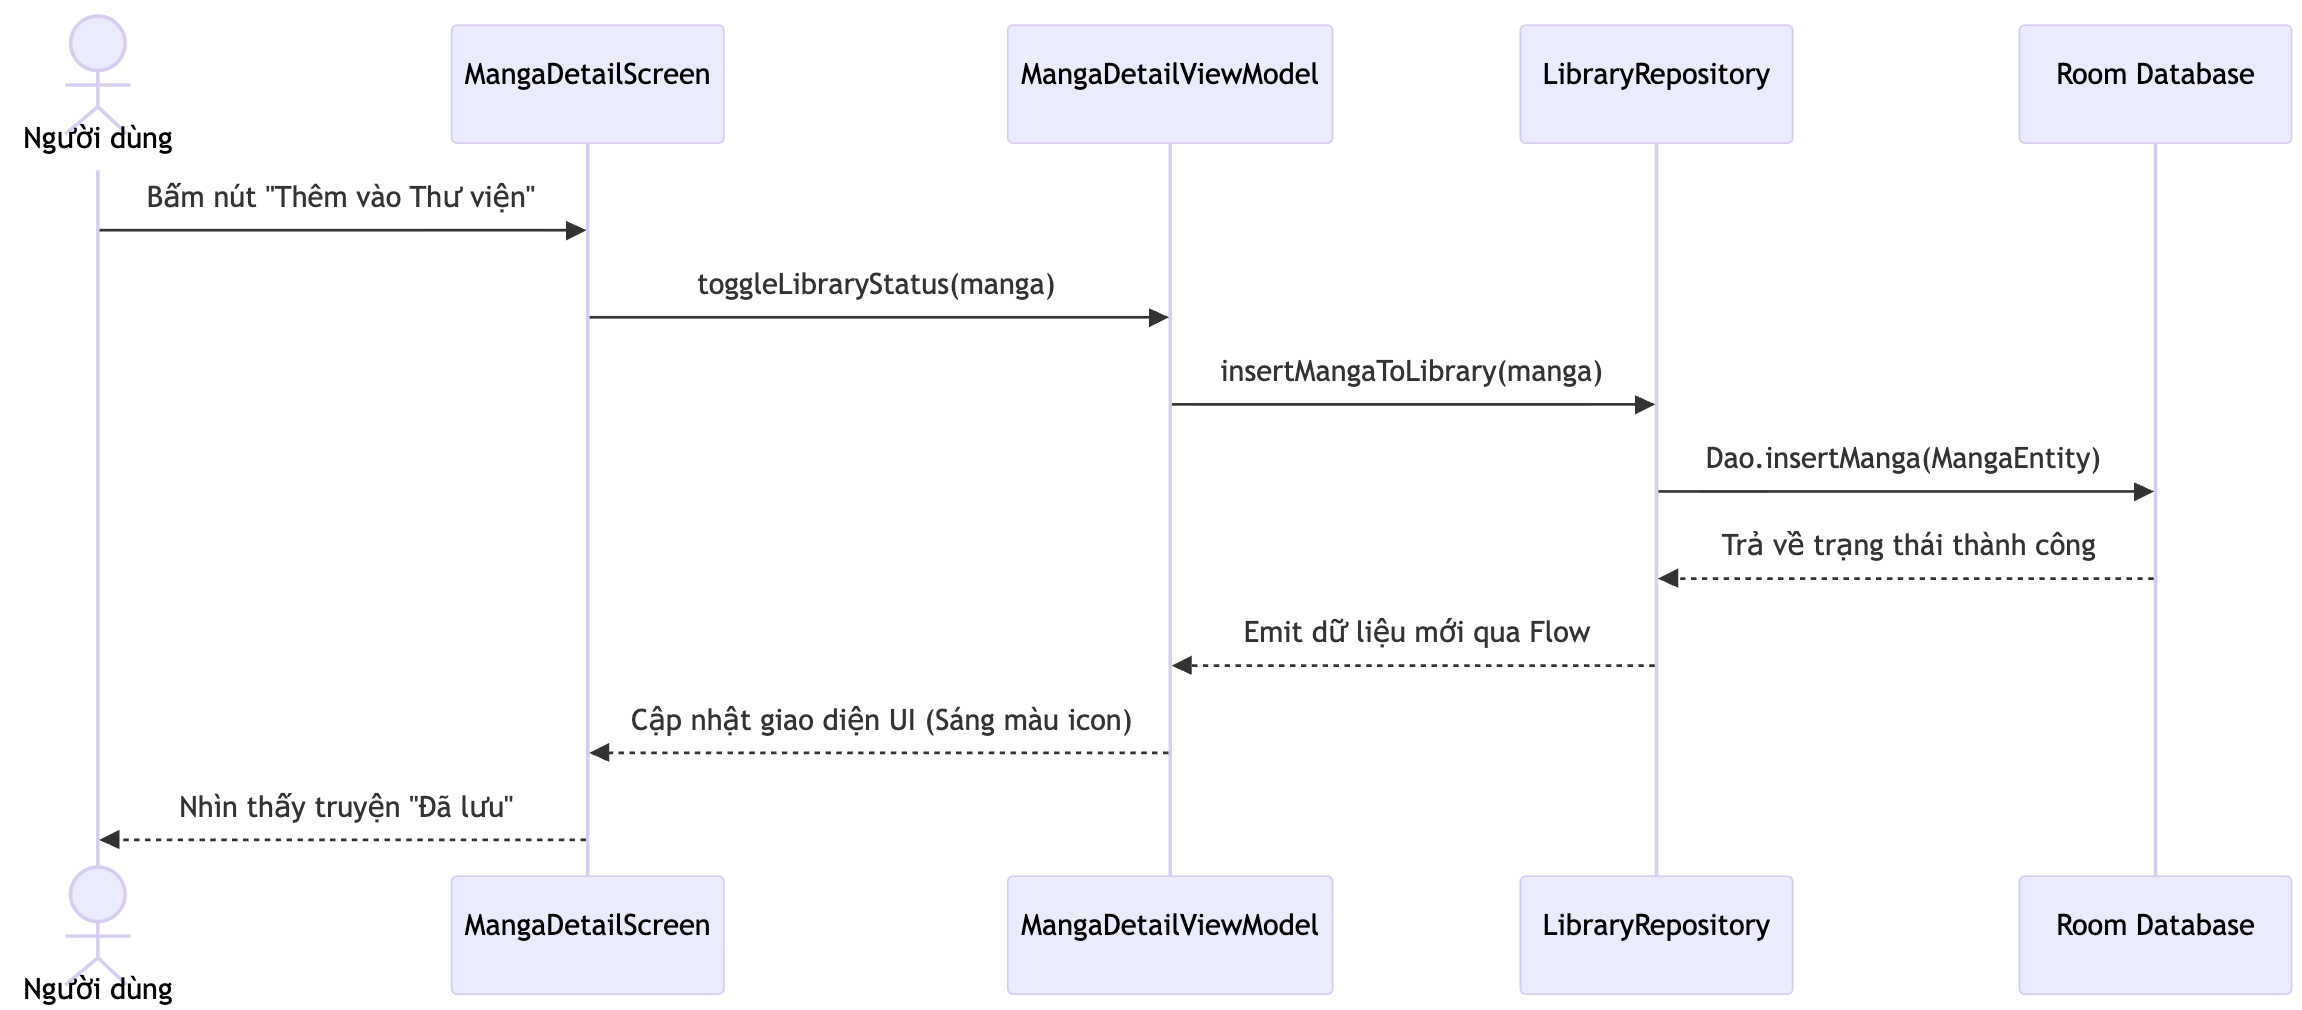
\includegraphics[width=0.9\textwidth]{figures/SaveBook.png}
    \caption{Sơ đồ tuần tự: Luồng lưu truyện vào thư viện cá nhân}
    \label{fig:seq_save_library}
\end{figure}

\textbf{Giải thích chi tiết:}
Room Database xử lý lưu trữ vào SQLite thành công. Do \texttt{ViewModel} luôn lắng nghe dữ liệu từ hàm \texttt{observeAll()} (trả về kiểu \texttt{Flow}), việc thay đổi dữ liệu trong database lập tức kích hoạt luồng phát ra dữ liệu mới. Trạng thái \texttt{isFavorite} được cập nhật, và giao diện UI tự động thay đổi (đổi màu biểu tượng trái tim) để báo hiệu thao tác lưu trữ thành công.

\section{Thiết kế Cơ sở dữ liệu cục bộ (Local Database)}

Để hỗ trợ khả năng lưu trữ thông tin và cho phép người dùng đọc truyện ngoại tuyến (offline) mà không cần phụ thuộc vào mạng, hệ thống sử dụng Room Database để quản lý cấu trúc cơ sở dữ liệu cục bộ.

\subsection{Sơ đồ Thực thể - Liên kết (ERD)}
Cơ sở dữ liệu được thiết kế xoay quanh các thực thể chính như \texttt{LibraryItemEntity} (Lưu trữ truyện yêu thích), \texttt{ChapterProgressEntity} (Lưu tiến trình đọc), \\ \texttt{ChapterMetadataEntity} (Siêu dữ liệu chương) và \texttt{DownloadQueueEntity} (Hàng đợi tải chương). Sơ đồ ERD dưới đây mô tả rõ ràng cấu trúc và mối quan hệ giữa các bảng:

\begin{figure}[H]
    \centering
    % TODO: Chèn ảnh Sơ đồ ERD Database
    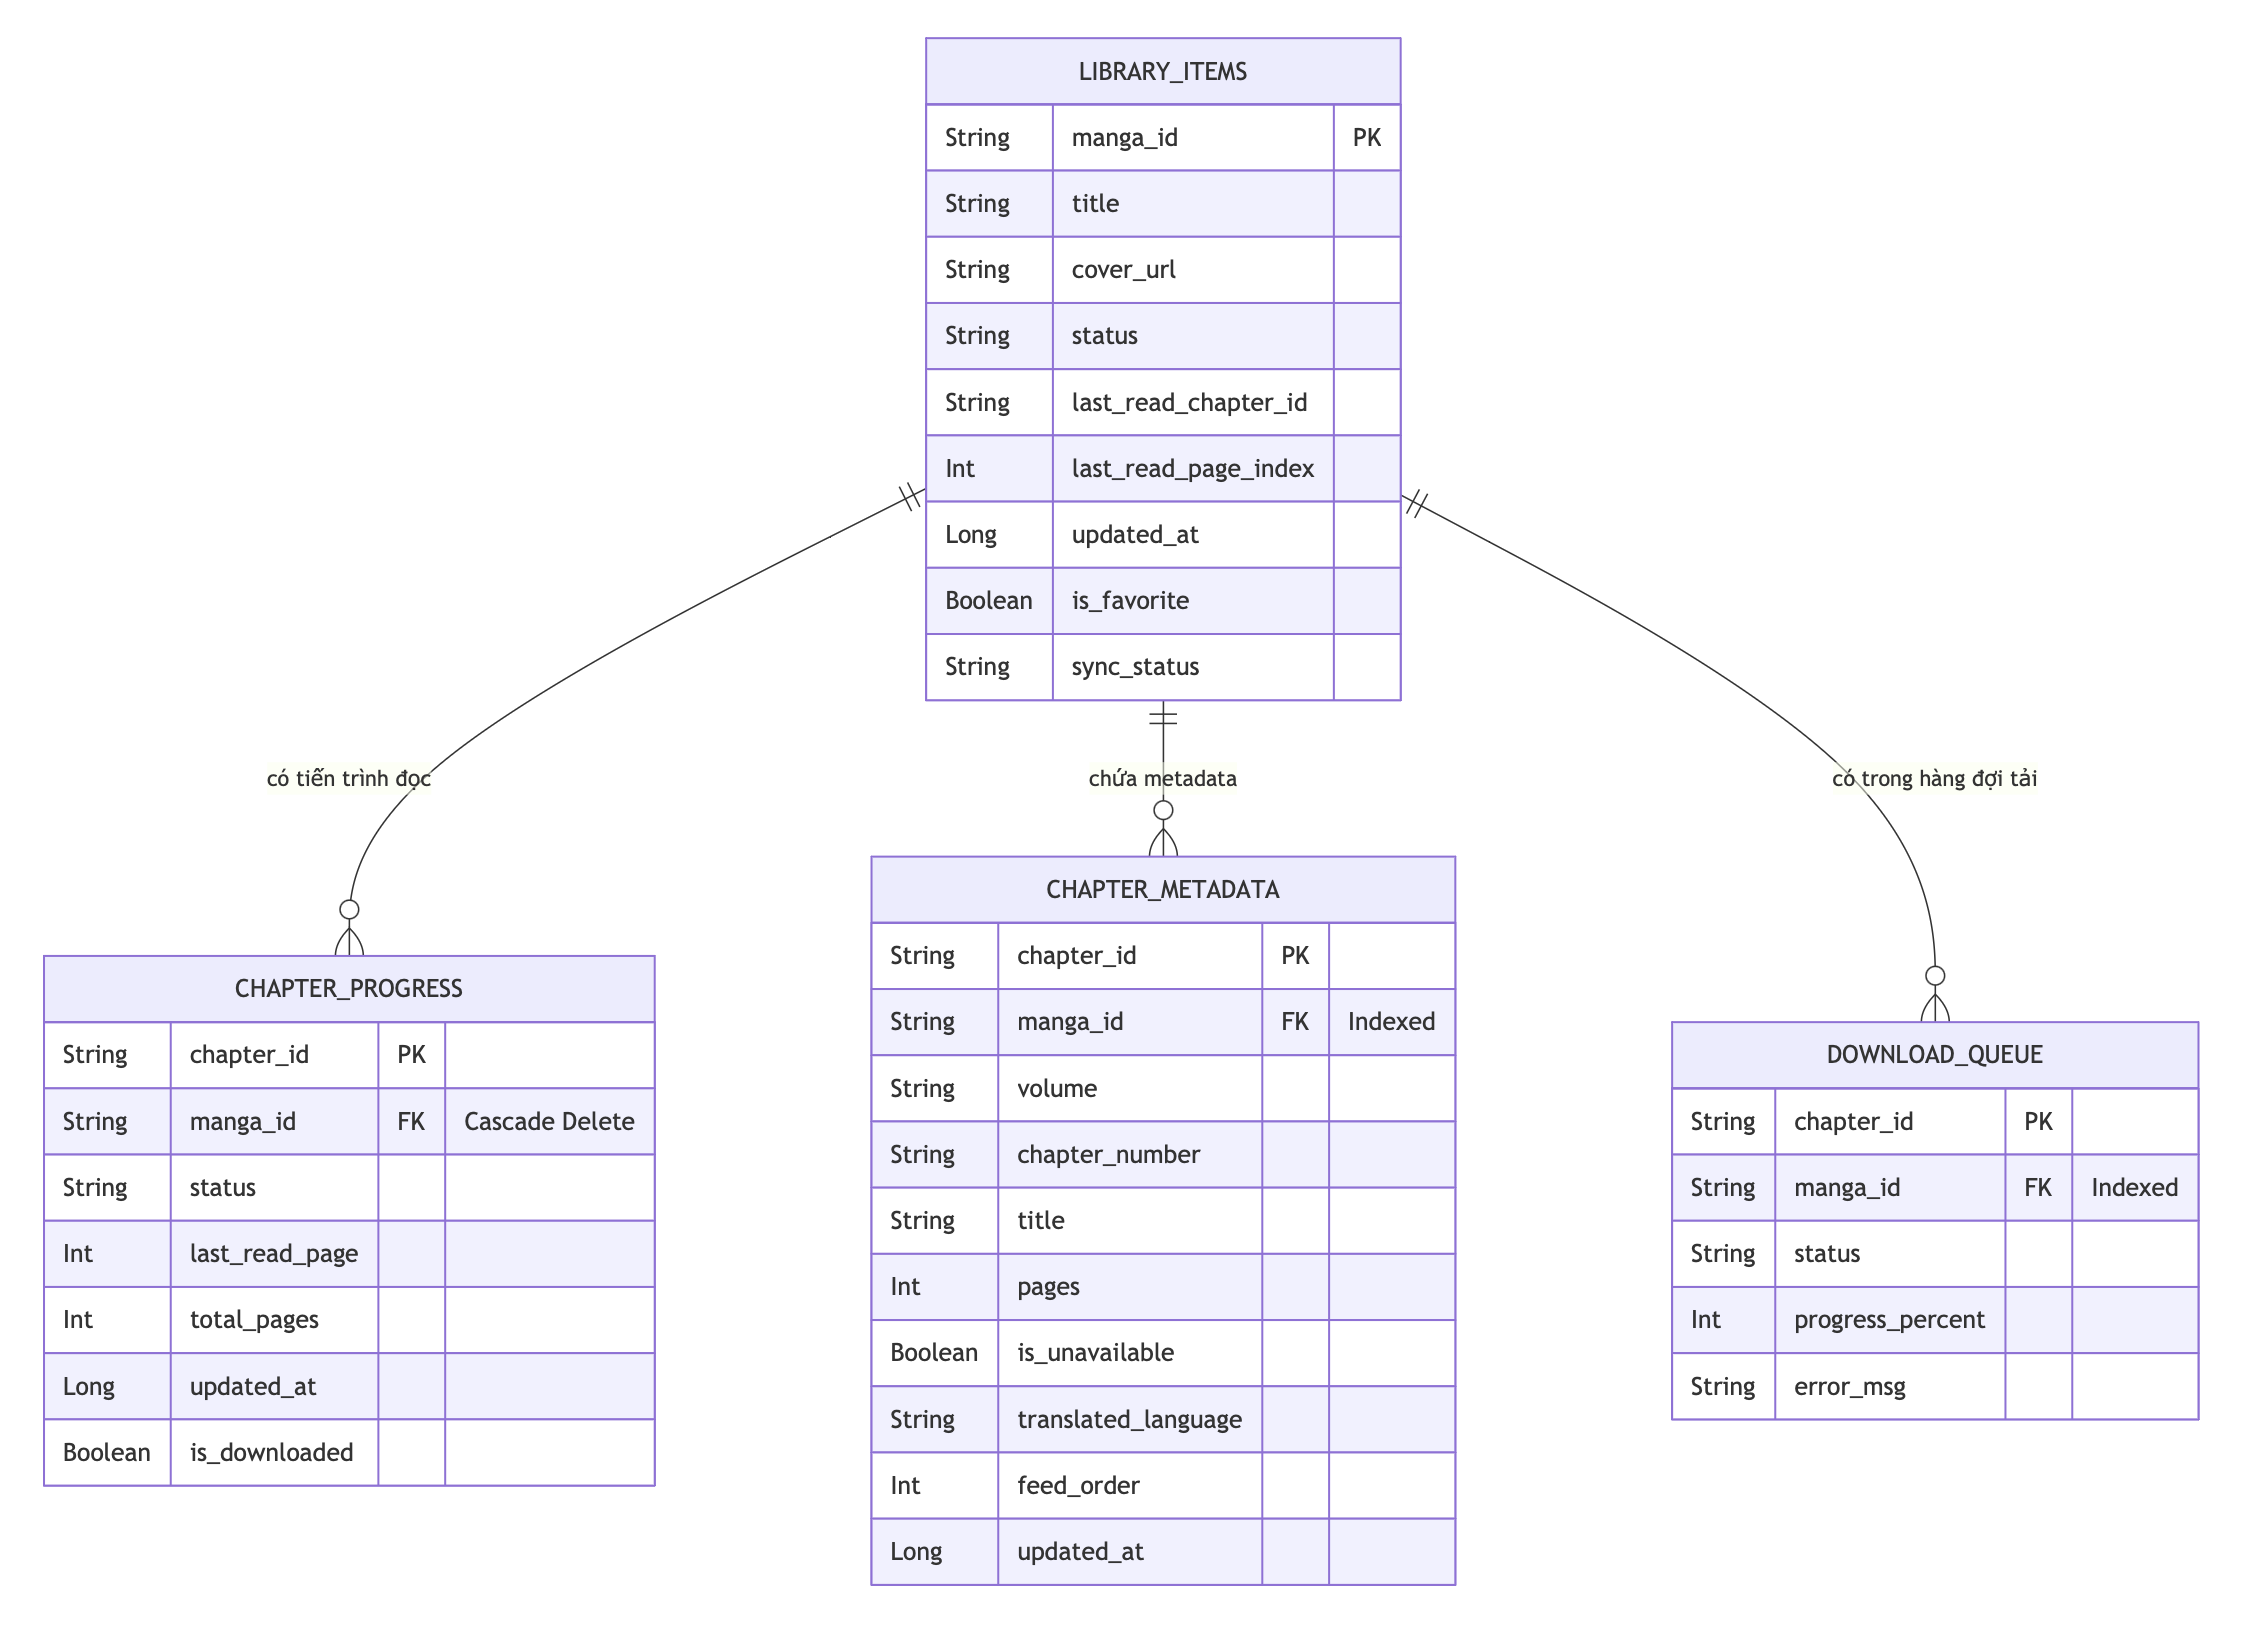
\includegraphics[width=0.9\textwidth]{figures/db_schema.png}
    \caption{Sơ đồ Thực thể - Liên kết (ERD) của cơ sở dữ liệu cục bộ}
    \label{fig:db_schema}
\end{figure}

% \subsection{Cài đặt mô hình bằng Room Database}
Ánh xạ dữ liệu được thực hiện thông qua các Data Class kết hợp với Annotation của Room. Hệ thống định nghĩa một Data Access Object (DAO). Các hàm truy vấn được thiết kế kết hợp chặt chẽ với \texttt{suspend} function và \texttt{Flow}, giúp giao diện luôn đồng bộ hóa theo thời gian thực.

% \begin{lstlisting}[language=Kotlin, caption={Định nghĩa các truy vấn dữ liệu thông qua LibraryDao}]
% @Dao
% interface LibraryDao {
%     @Upsert
%     suspend fun upsert(item: LibraryItemEntity)

%     // Lang nghe danh sach truyện yêu thích liên tuc để cap nhat UI
%     @Query("SELECT * FROM library_items WHERE is_favorite = 1 ORDER BY updated_at DESC")
%     fun observeFavorites(): Flow<List<LibraryItemEntity>>

%     @Query("DELETE FROM library_items WHERE manga_id = :mangaId")
%     suspend fun deleteByMangaId(mangaId: String)
% }
% \end{lstlisting}
\subsection{Chiến lược lưu trữ dữ liệu tải về (Offline Storage)}

Để tối ưu hóa hiệu năng, hệ thống áp dụng chiến lược phân tách giữa "Dữ liệu trạng thái" (State Data) và "Dữ liệu nhị phân" (Binary Data) cho tính năng tải truyện:

\begin{itemize}
    \item \textbf{Quản lý trạng thái bằng SQLite:} CSDL Room chỉ quản lý hàng đợi tải (\texttt{DownloadQueueEntity}) và lưu cờ trạng thái \texttt{is\_downloaded} trong \\ \texttt{ChapterProgressEntity}. Việc này giúp tránh lưu trữ file ảnh lớn (BLOB) trực tiếp vào SQLite, ngăn chặn tình trạng tràn bộ nhớ \\ (\texttt{CursorWindowAllocationException}) và giữ CSDL luôn gọn nhẹ.
    \item \textbf{Lưu trữ file vật lý (Internal Storage):} Các trang truyện thực tế được lưu trực tiếp dưới dạng tệp tin ảnh vào bộ nhớ trong của thiết bị với đường dẫn cô lập: \texttt{/files/offline\_manga/\{manga\_id\}/\{chapter\_id\}/}. Tại mỗi thư mục chương sẽ lưu các trang ảnh và một tệp \texttt{.complete} để xác nhận chương đã tải toàn vẹn.
\end{itemize}

\section{Kiến trúc quản lý tài khoản và đồng bộ đám mây (Firebase)}

Để tối ưu hóa chi phí vận hành đám mây và nâng cao trải nghiệm người dùng, hệ thống không sử dụng mô hình cơ sở dữ liệu quan hệ truyền thống mà áp dụng mô hình kiến trúc hướng tài liệu (Document-Oriented NoSQL) trên \textbf{Firebase Cloud Firestore}, kết hợp với \textbf{Firebase Authentication}.

\subsection{Xác thực và Phân vùng dữ liệu theo UID}
Sau khi \textbf{Firebase Authentication} xác thực người dùng thành công và cấp một mã \texttt{UID} duy nhất, mã này đóng vai trò là gốc (Root Key) cho mọi truy vấn dữ liệu từ xa. Toàn bộ dữ liệu cá nhân hóa của người dùng không nằm chung một bảng lớn mà được phân rã thành các bộ sưu tập con (Sub-collections) độc lập, cô lập hoàn toàn theo \texttt{UID}. Cấu trúc cây dữ liệu được tối ưu hóa như sau:

\begin{itemize}
    \item \path{users/{UID}/favorite_mangas/{manga_id}}: Lưu trữ danh sách truyện yêu thích.
    \item \path{users/{UID}/reading_progress/{chapter_id}}: Lưu chi tiết tiến trình đọc (vị trí trang dở).
\end{itemize}

Cách thiết kế NoSQL phân cấp này là tối ưu nhất vì nó loại bỏ hoàn toàn các thao tác lọc dữ liệu (\texttt{Filter/Query}) tốn kém trên Cloud. Mỗi thiết bị chỉ truy cập trực tiếp vào đúng phân vùng của mình thông qua đường dẫn trực tiếp chứa \texttt{UID}.

\subsection{Cơ chế đồng bộ tối ưu (Offline-First Sync)}
Mối tương quan giữa cơ sở dữ liệu cục bộ (Room) và đám mây (Firebase) được thiết kế theo mô hình lai nhằm tối ưu hóa băng thông mạng:

\begin{enumerate}
    \item \textbf{Single Source of Truth (SSOT):} Room Database tại local đóng vai trò là nguồn dữ liệu duy nhất điều khiển giao diện UI. Khi người dùng nhấn thích truyện hoặc đọc đến một trang mới, ứng dụng sẽ lập tức cập nhật vào Room (\texttt{library\_items} và \texttt{chapter\_progress}) để đảm bảo phản hồi giao diện ngay lập tức mà không phụ thuộc vào tốc độ mạng.
    \item \textbf{Đồng bộ hóa bất đối xứng:} Khi thiết bị có kết nối mạng ổn định, tầng Data Layer (Repository) sẽ kích hoạt luồng đồng bộ đẩy các bản ghi có sự thay đổi trạng thái (\texttt{sync\_status = PENDING}) lên phân vùng tương ứng trên Firebase. 
    \item \textbf{Tối ưu hóa lượt đọc/ghi (Read/Write):} Tiến trình đọc dở trong một chương (\texttt{last\_read\_page\_index}) thay vì đẩy liên tục lên đám mây theo từng giây người dùng lật trang, hệ thống chỉ thực hiện đồng bộ khi người dùng thoát chương, bấm dừng hoặc theo chu kỳ thời gian (Debounce/WorkManager). Cơ chế này giúp giảm tới 80\% chi phí số lần gọi API lên Firebase Cloud.
\end{enumerate}

\section{Thiết kế Trải nghiệm Người dùng (UX/UI) và Tính tương thích}

Do đặc thù của ứng dụng đọc truyện tranh, giao diện hiển thị yêu cầu sự linh hoạt cao để tối ưu hóa không gian đọc cho người dùng. Các tiêu chí thiết kế được đảm bảo bao gồm:

\begin{itemize}
    \item \textbf{Khả năng đáp ứng (Responsive Design):} Giao diện được thiết kế để tự động thay đổi bố cục linh hoạt trên các kích thước màn hình khác nhau. Ví dụ khi xoay ngang màn hình, thành pill navigation bottom bar được chuyển sang bên.
    \item \textbf{Xử lý thay đổi cấu hình (Configuration Changes):} Hệ thống hỗ trợ xoay màn hình (Portrait/Landscape) mượt mà, đảm bảo không cần gọi lại API hay truy vấn lại cơ sở dữ liệu. 
\end{itemize}